\begin{ReasoningBox}[title=Event Prediction] % 可以通过 title 参数修改标题
    % --- 第一部分：问题描述与图片 ---
    % \begin{minipage}[t]{0.58\textwidth}
    
        \textbf{Question:} Your task is to predict whether it will rain or not in New York in the next 24 hours. Review the time-series data provided for the last 24 hours. Each time series consists of hourly values separated by a '|' token for the following indicators:

    \vspace{0.5em}
    \begin{wrapfigure}{r}{0.5\textwidth}
        \centering
        % wrapfigure 通常顶部会有多余空白，使用负 vspace 向上提，让图片和第一行文字对齐
        \vspace{-20pt} 
        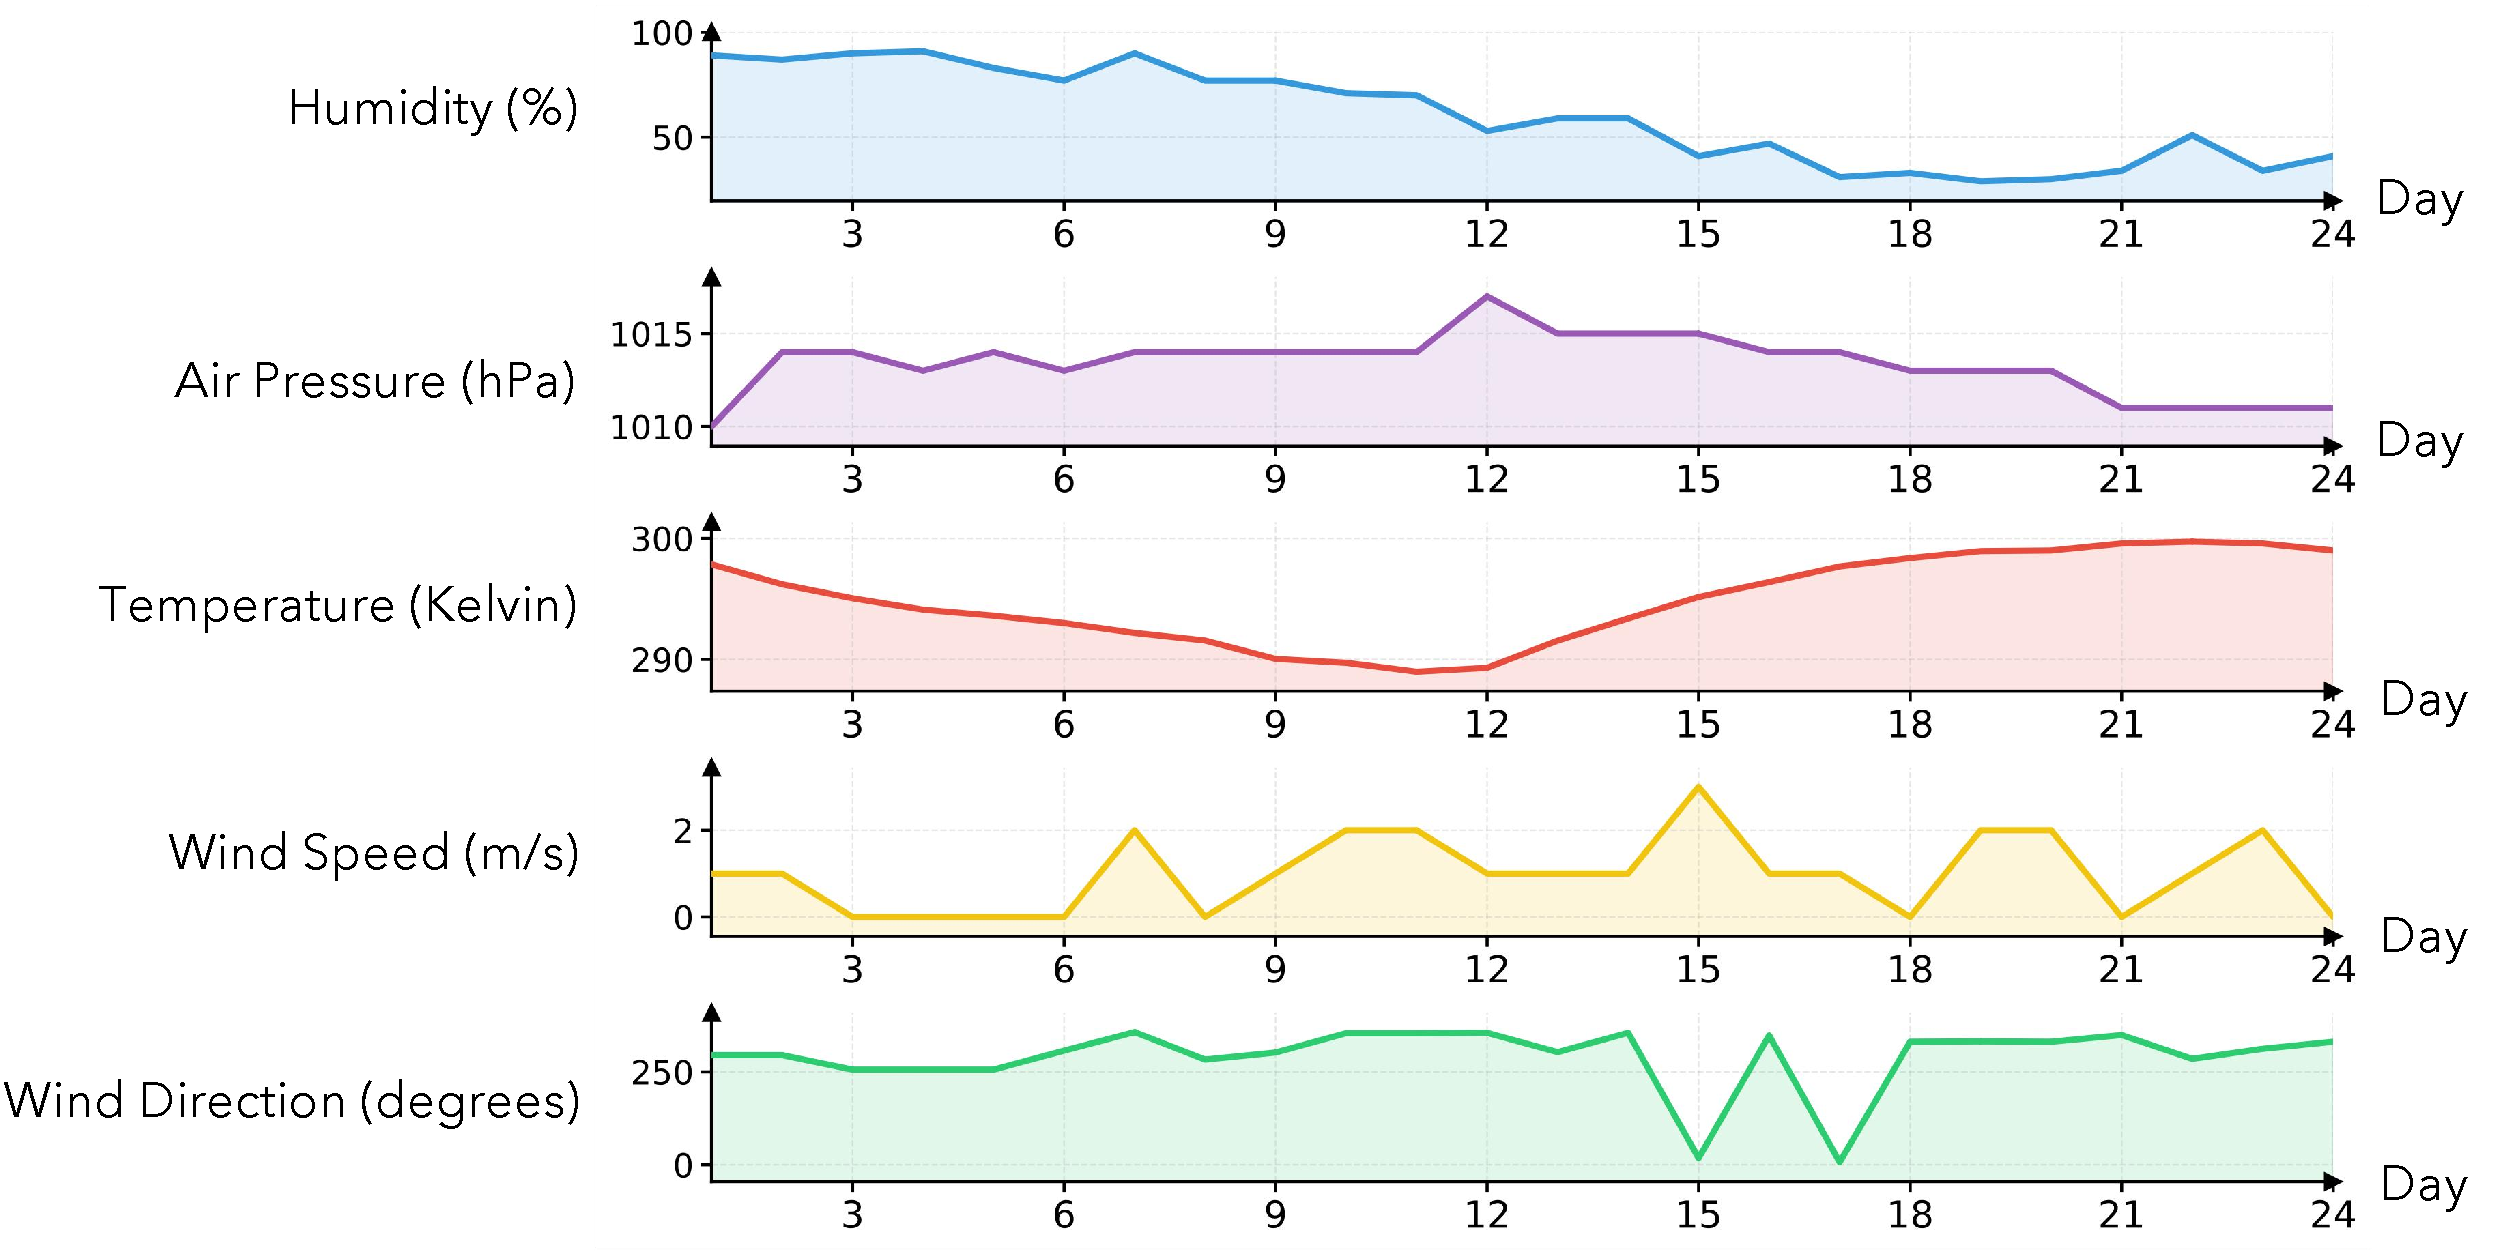
\includegraphics[width=\linewidth]{blocks/sample_cases_success/event.pdf}
        % 调整底部的留白
        % \vspace{-20pt}
    \end{wrapfigure}
    % --- 第二部分：选项 ---
    \textbf{Answer Choices:} \\
    (A) Rain \\
    (B) No Rain \\
    \textbf{Correct Answer:} \textcolor{correctgreen}{(B)} \\
        
    \vspace{5.5em}
\end{ReasoningBox}